\documentclass[10pt,a4paper]{article}

%double si on veut une version prof et une version élève. simple si on veut une seule version.
\newcommand{\buildmode}{double}

\InputIfFileExists{version.tex}{}{}
% Version (définie par le script)
\providecommand{\version}{eleve}

\usepackage{feuilleexo}
\usepackage{schemaevolution}

%%%à modifier à chaque fois

\renewcommand{\niveau}{1M}
\renewcommand{\chapitre}{Évolutions et évolutions successives}
\renewcommand{\numchap}{0.2} 
\renewcommand{\theme}{Statistiques}

\begin{document}


%\legendeicones

\vspace{-0.3cm}

\begin{prerequis}
\begin{itemize}
    \item Savoir calculer avec des fractions.
    \item Passer d'une écriture décimale à une écriture fractionnaire et inversement.
\end{itemize}

\end{prerequis}

\prof{
    Première partie : l'objectif est de comprendre la notion d'évolution et de savoir les calculer dans des cas simples (fractions remarquables). Au tableau, rappeler l'enjeu. Faire plusieurs schémas au tableau et les faire compléter par les élèves.
}

\begin{multicols}{2}
\section{Calculer avec des évolutions simples}

\begin{exo}[][]
    \begin{enumerate}
        \item Compléter les schémas suivants :
            \schemaevolution{20}{\dots}{50\%}{}
            \schemaevolution{60}{\dots}{-20\%}{}
            \schemaevolution{2}{\dots}{100\%}{}
            \schemaevolution{80}{100}{\dots}{}
        \item Retrouver la quantité manquante dans chacun des cas : \begin{enumerate}
            \item Une population de 2000 habitants a augmenté de 25\%. Quelle est la population finale ?
            \item Un produit qui coûtait 80€ a vu son prix passer à 88 euros. Quel est le pourcentage d'augmentation ?
            \item Un jean qui coûtait 50€ a diminué de 40\%. Quelle est la nouvelle prix ?
        \end{enumerate}
    \end{enumerate}
\end{exo}


\prof{
    Enchaîner sur le cours ensuite pour introduire la méthode générale pour calculer des évolutions. Donner toutes les formules. 
}

\section{Évolutions et coefficient multiplicateur}

\begin{exo}
    Une veste coûte 140 euros. Lors d'une promotion, son prix diminue de 30\%.\begin{enumerate}
        \item Calculer le coefficient multiplicateur associé à cette évolution.
        \item En déduire le nouveau prix de la veste.
        \item Complétez le schéma ci-dessous :
        \schemaevolution{\dots }{\dots}{-\dots \%}{ \times \dots}
    \end{enumerate}
\end{exo}

\begin{exo}
    Compléter le tableau suivant :
    \medbreak
    \begin{tabular}{|c|c|}
        \hline
        \textbf{Taux d'évolution} & \textbf{Coefficient multiplicateur} \\ \hline
                & 1,32  \\ \hline
         + 15\% &       \\ \hline
                & 0,8   \\ \hline
           -5\% &       \\ \hline
           +2\% &       \\ \hline
                & 2,3   \\ \hline

    \end{tabular}
\end{exo}

\begin{exo}
    M. Levifve veut acheter le moins cher de ces trois maillots pour l'annniversaire de M. André. Lequel va-t-il acheter ?
    \begin{center}
    \begin{multicols}{3}
    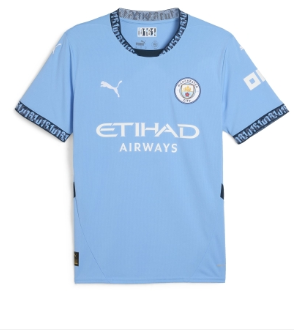
\includegraphics[height=0.1\textwidth]{img_maillots/img1.png}\\
    \st{80,00 \euro}\\
    -20\%

    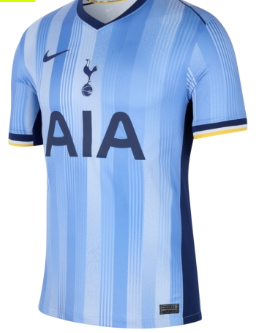
\includegraphics[height=0.1\textwidth]{img_maillots/img2.png}\\
    \st{70,00 \euro}\\
    -15\%

    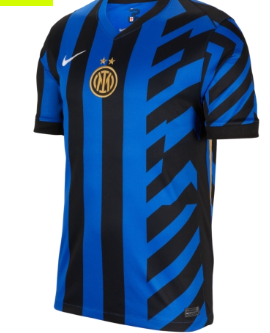
\includegraphics[height=0.1\textwidth]{img_maillots/img3.png}\\
    \st{90,00 \euro}\\
    -34\%
    \end{multicols}
    \end{center}
\end{exo}

\prof{
    Pour la correction, penser à faire un schéma dans chacun des cas.
}

\begin{exo}
    Une entreprise comptait 350 milliers d'euros de chiffre d'affaire au premier janvier 2026. en 6 mois, ce nombre est passé à 322 milliers d'euros. De quel pourcentage le chiffre d'affaires a-t-il baissé ?
\end{exo}

\begin{exo}
    En 2025, le budget de l'état consacré à la défense était de 50 milliards d'euros. Ce budget a augmenté de 7 milliards d'euros supplémentaires en 2026. Quel sera le pourcentage d'évolution de ce budget entre ces deux années ?
\end{exo}


\section{Evolutions successive}

\begin{exo}
Compléter les schémas suivants :


\schemaDeuxevolutions{200}{\dots}{\dots}{1,4}{}{}{}{}{}
\end{exo}

\begin{exo}[Avec calulatrice][]
    
    Ce graphique représente l'évolution de la démographie en Seine-Saint-Denis (source : Wikipedia).
\begin{center}
    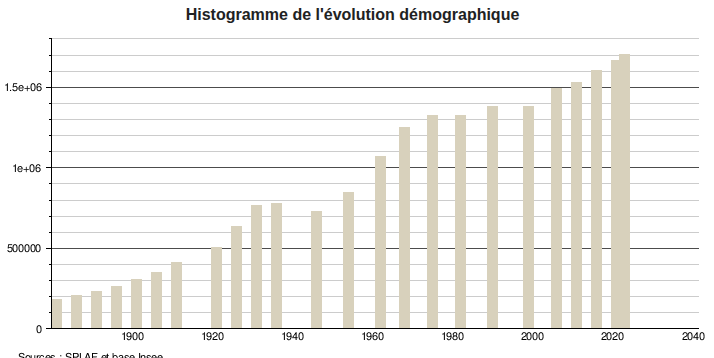
\includegraphics[width=0.5\textwidth]{population_saint_denis.png}
\end{center}

\begin{enumerate}
    \item Combien y avait-il d'habitants en 1980 ? En 2023 ?
    \item En déduire l'évolution de la population entre 1980 et 2023, en pourcentage.
\end{enumerate}
\end{exo}
\end{multicols}

\end{document}
